\chapter{Architectuur}

Zoals beschreven in vorige secties gaan we een library ontwikkelen om applicaties te kunnen monitoren. Tracklytics is de naam van de library en wordt in het vervolg van dit document gebruikt om de library aan te duiden. \\
In deze sectie worden de architecturale beslissingen die gemaakt zijn uit de doeken gedaan.  \\


Zoals getoond op de volgende figuur \ref{fig:component} bestaat de Tracklytics library uit vier verschillende componenten:
\begin{itemize}
\item UserApplication: De applicatie die de developer wil monitoren
\item TracklyticsCore: Stelt de library voor waarmee de UserApplication communiceert om te kunnen monitoren.
\item TracklyticsBackend: De backend die de informatie verwerkt die van de TracklyticsCore komt.
\item Dashboard: Een dashboard om alle informatie weer te geven.
\end{itemize}

Deze componenten vormen samen de core van de Tracklytics library. Deze communiceren onderling via de aangeboden interfaces. In de rest van dit hoofdstuk worden deze componenten beschreven en worden de architecturale beslissingen uitgelegd met een motivatie waarom die beslissingen gemaakt zijn.

\begin{figure}[!h]
  \centering
  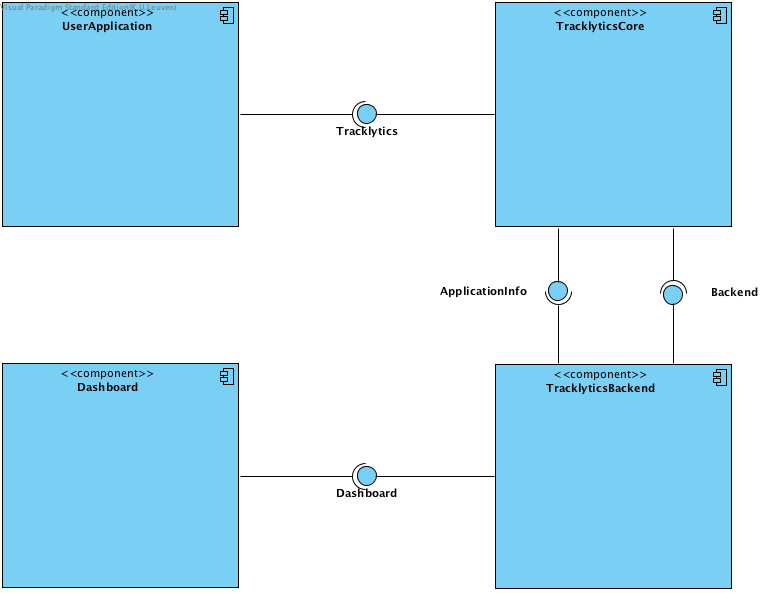
\includegraphics[scale=0.4]{Afbeeldingen/Architectuur/Component}
  \caption{Component diagram Tracklytics library.}
  \label{fig:component}
\end{figure}

\section{Component Diagram}
Het component diagram \ref{fig:component} duidt aan welke componenten een rol spelen in het bouwen van de Tracklytics library. In de volgende secties worden de verschillende componenten beschreven en hun rol wordt uitgelegd.





\subsection{UserApplication}
De UserApplication component representeert een applicatie ontwikkeld door developers. De UserApplication gebruikt de Tracklytics interface om metingen uit te voeren en de applicatie te monitoren. Developers moeten zelf aangeven welke elementen er gemonitord moeten worden. 


\subsection{TracklyticsCore}
De TracklyticsCore component stelt een monitoring library voor die in deze thesis ontwikkeld wordt. De TracklyticsCore component verzamelt informatie die hij doorkrijgt van de UserApplication component, slaat deze tijdelijk op het toestel op om deze dan later, na een bepaald tijdsinterval, door te sturen naar de TracklyticsBackend component via de Backend interface.  \\

\paragraph{Interface}
De TracklyticsCore component biedt een Tracklytics interface aan. De UserApplication kan deze interface gebruiken om de applicatie te monitoren. De TracklyticsCore stuurt deze data door naar de server.\\

De interface bestaat uit methodes om de applicatie te monitoren. Tracklytics biedt vijf elementen aan om de applicatie te kunnen monitoren, namelijk:
\begin{itemize}
\item Counter: Kan gebruikt worden om evenementen te tellen
\item Meter: Kan gebruikt worden om periodiek waardes op te halen.
\item Histogram: Kan gebruikt worden om een waarde te verzamelen dat in het dashboard in een histogram gegoten kan worden. 
\item Timer: Kan gebruikt worden om de lengte van een evenement te meten.
\item Gauge: Kan gebruikt worden om een bepaalde waarde te meten. 
\end{itemize}

Deze elementen vormen de kern van de Tracklytics library en worden verder besproken in het volgende hoofdstuk om duplicatie van tekst te vermijden \ref{sec:Klassediagram}. \\


\subsection{TracklyticsBackend}
De TracklyticsBackend component representeert de server kant van de library. Hierop draait de code om de gemonitorde data op te slaan in de database. De TracklyticsBackend component bevat dus de database om alle informatie in op te slaan. \\
De TracklyticsBackend component biedt drie interfaces aan, namelijk: ApplicationInfo, Backend en Dashboard. Deze worden in de volgende paragrafen besproken.\\

\subsubsection{Interfaces}
\paragraph{ApplicationInfo}
Deze interface wordt gebruikt door de TracklyticsCore om instellingen van de developer op te halen die gemaakt zijn in het dashboard, zoals bv. bij het On Demand aan- of uitzetten van het monitoren zoals iets verder besproken \ref{par:OnDemand}.

\paragraph{Backend}
Deze interface wordt gebruikt om data uit te wisselen tussen de TracklyticsCore en de TracklyticsBackend. Dit is de gemonitorde data die de TracklyticsCore verzameld heeft. De TracklyticsBackend verwerkt deze informatie en slaat deze op in de database.\\

\paragraph{Dashboard}
Deze interface wordt gebruikt door het dashboard om de data uit de database op te halen om deze weer te kunnen geven aan de developers. 

\subsection{Dashboard}
De Dashboard component representeert een applicatie om de gemonitorde data van de Tracklytics library weer te kunnen geven aan de developers en de eigenaars. Met behulp van grafieken en verwerkte data kunnen de developers en de eigenaars beslissingen nemen omtrent de applicatie.\\


\begin{figure}[!h]
  \centering
  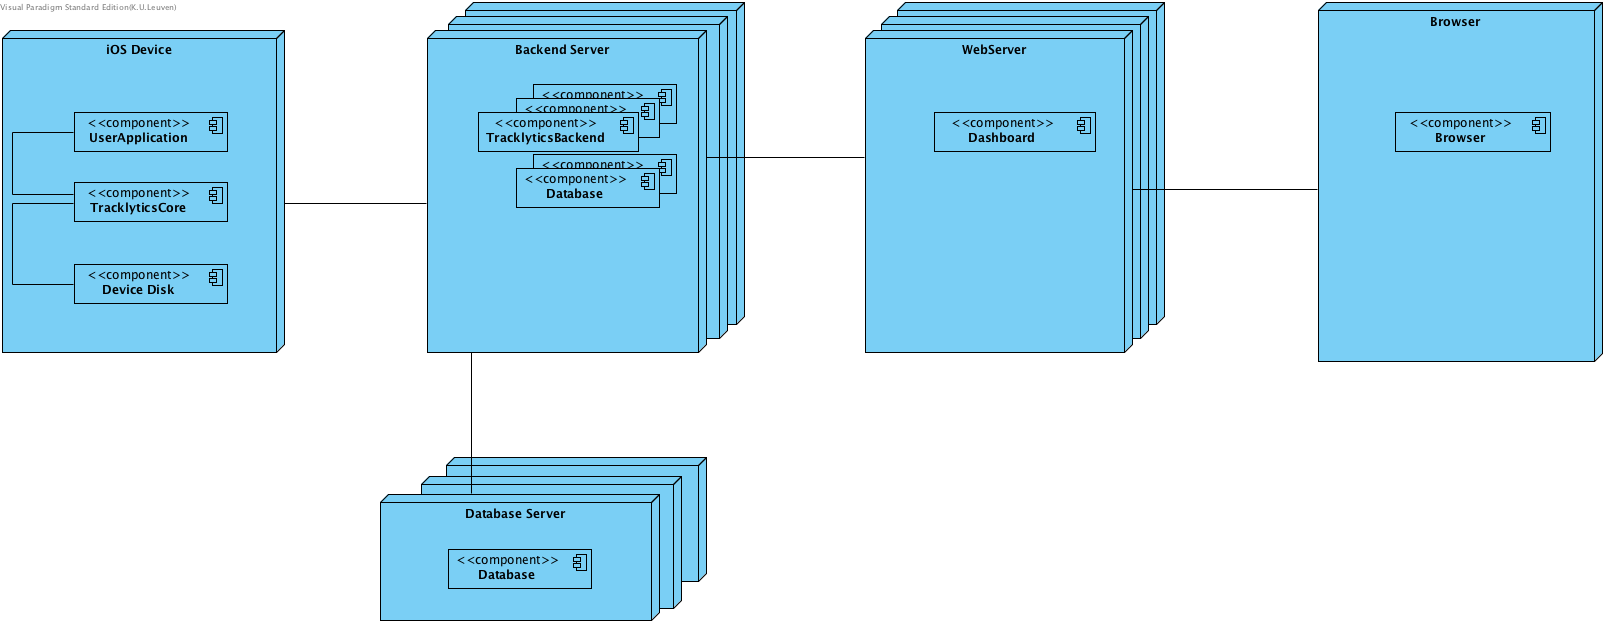
\includegraphics[scale=0.30]{Afbeeldingen/Architectuur/Deployment}
  \caption{Deployment diagram Tracklytics library.}
  \label{fig:deployment}
\end{figure}
\section{Deployment Diagram}
Het deployment diagram toont op welke nodes de componenten besproken in vorige sectie draaien. Zoals je kan zien draait de UserApplication en de TracklyticsCore op het mobiele toestel van de gebruiker zelf. De TracklyticsBackend draait op een backend server die gerepliceerd kan worden. Deze staat in verbinding met een Database server waar alle data wordt opgeslagen. Het Dashboard draait op een webserver. Deze staat in verbinding met de backend server om de data te kunnen ophalen.

\section{Uitbreidingen}
In deze sectie worden een aantal uitbreidingen besproken die niet standaard in een monitoring library zitten, maar zeer handig kunnen zijn om developers te helpen bij het monitoren van de applicatie.

\paragraph{Data availability}
Smartphones vallen weleens zonder internet connectiviteit door het wegvallen van een WiFi verbinding of het wegvallen van de mobiele verbinding. De Tracklytics library zendt de gemonitorde data over het internet naar de backend om deze op te slaan in een database. Als de internetverbinding zou wegvallen, dan zou er mogelijks belangrijke data verloren gaan. Om dit scenario te voorkomen slaan we de data tijdelijk op op de harde schijf van de mobiele telefoon. Indien de smartphone dan terug verbinding met het internet heeft gemaakt kan de data alsnog gesynchroniseert worden met de backend. De data wordt tijdelijk opgeslagen, dus nadat de data gesynchroniseerd is wordt deze van de smartphone verwijderd. Zo wordt ervoor gezorgd dat de data in ieder geval in de database terecht komt. 

\paragraph{On Demand}\label{par:OnDemand}
Het is de bedoeling de developer zoveel mogelijk vrijheid te geven in het monitoren van de applicatie. Om deze vrijheid te verhogen is het On Demand aan- of uitzetten van het monitoren aan Tracklytics toegevoegd. Een developer kan vanuit het dashboard aangeven of de applicatie op dit moment gemonitord moet worden of niet. Dit kan gebruikt worden om op de piekdagen of piekmomenten het monitoren aan te zetten. Zo kan uitgezocht worden of er een bottleneck bestaat als het gebruik van de applicatie piekt. \\
Indien een developer ontdekt dat er geen bottleneck of problemen zijn met de app en deze niet verder gemonitord moet worden, dan is het handig om de monitoring uit te kunnen zetten. Dit zorgt ook voor een prestatieboost, omdat er niet meer gesynchroniseerd moet worden naar de server en de data moet niet meer op het toestel verwerkt en opgeslagen worden door Tracklytics.


\paragraph{Aggregatie}
De data die doorgestuurd wordt naar de server zegt op zichzelf niets. Om een goede analyse weer te geven in het dashboard moet deze data geaggregeerd worden. Er zijn twee plaatsen waar deze aggregatie uitgevoerd kan worden, namelijk op de smartphone zelf in de Tracklytics library of in de backend. \\
De reden om de aggregatie op de smartphone uit te voeren is dat er hiermee al een deel van de verwerking gedaan wordt en de backend bij het opvragen van de data vanuit het dashboard minder werk heeft om deze samen te voegen en verwerken. Er is dus een prestatiewinst langs de serverkant indien de aggregatie op de smartphone uitgevoerd wordt. 
Een nadeel is dat deze aggregatie meer CPU tijd van de smartphone gebruikt dan als we de aggregatie in de backend uitvoeren en dit kan ervoor zorgen dat de applicatie traag gaat overkomen bij de gebruikers. Er is dus een goede afweging nodig waar deze aggregatie gebeurt.\\

Een functie in het dashboard zou ervoor kunnen zorgen dat de developer de optie krijgt om te kiezen of deze aggregatie op de telefoon of in de backend uit te voeren. Dit geeft de developer ook weer meer vrijheid om deze keuzes te maken.

\paragraph{AB Testing}
AB testing is een mechanisme dat grote bedrijven, zoals facebook, gebruiken om nieuwe features uit te rollen naar de gebruikers. Het mechanisme werkt als volgt: er bestaat een versie A en een versie B van de software met B de nieuwere versie. AB testing zorgt ervoor dat de uitrol van versie B geleidelijk verloopt. De gebruikers van de software worden dus in twee (of meerdere) groepen opgedeeld door een bepaalde eigenschap. Deze eigenschap kan vanalles zijn, namelijk: geografische locatie, ingestelde taal, de gebruikte browser, het type toestel, enz. Indien er dan een probleem met versie B is, dan bestaat dit enkel bij de groep die versie B al verkregen is en dus niet bij alle gebruikers. Hierdoor merkt enkel die groep dat er een probleem is en kan versie B aangepast worden om dit probleem op te lossen of eventueel kan ervoor gezorgd worden dat iedereen terug versie A gebruikt tot het probleem in versie B opgelost is. \\

In mobiele applicaties is het moeilijker om echt aan AB testing te doen, omdat deze applicaties meestal statisch zijn, er moet een update in de app store komen om een nieuwe versie met nieuwe features en code uit te rollen. Dit staat pal tegenover websites die hun webpaginas en code rechtstreeks van een server halen en waar de aanpassingen aan de versies meteen zichtbaar zijn bij de gebruikers. 
Een workaround van dit probleem is dat de mobiele applicatie de code van de nieuwe versie (B) al kan bevatten en ook nog de code van de oude versie (A) erin heeft staan. Tracklytics kan dan een functie in het dashboard aanbieden om de groepen op te delen in twee (of meerdere) groepen op basis van eigenschappen die de developer kan kiezen. In de mobiele applicatie moeten we dus dat onderscheid kunnen maken welke code aangeroepen moet worden. Het gemakkelijkste is om een codenaam aan de versie toe te voegen, zodat er meerdere versies van de code aanwezig kan zijn. 
Het nadeel van dit mechanisme is dat de applicatie groter is dan hij zou zijn moest de applicatie enkel de code bevatten die voor die bepaalde groep nodig is.


\paragraph{Security \& Privacy}
Een belangrijk aspect is de privacy van de gebruiker. Zoals eerder al aangehaald is NewRelic een closed source library, wat wil zeggen dat developers niet weten welke informatie er doorgestuurd wordt naar de backend. Dit gegeven zorgt ervoor dat privacygevoelige applicaties deze library niet zouden mogen gebruiken, omdat er gebruikersinformatie gelekt zou kunnen worden naar de backend van NewRelic zoals bijvoorbeeld email-adressen, creditcard gegevens, etc.\\
Om deze reden is ervoor gekozen dat Tracklytics open source is. Zo kunnen developers zeker zijn welke informatie er wordt doorgestuurd naar de backend en is de privacy van de gebruiker wel gegarandeerd. Tracklytics verzamelt enkel metadata van de telefoon en de applicatie. De metadata die gecollecteerd wordt door Tracklytics bestaat uit: het type toestel, de versie, de naam van de applicatie, een identifier van de applicatie, een identifier van het toestel om deze van elkaar te kunnen onderscheiden, de datum en het type connectie waarop het toestel zich bevindt. Dit gegeven zorgt ervoor dat Tracklytics de privacy van de gebruiker garandeert..\\

Naast privacy is security ook een belangrijk aspect. Er bestaat namelijk een verbinding tussen de mobiele applicatie en de backend over een onveilig netwerk. Het zou dus niet mogen dat de doorgezonden data door een onrechtmatig iemand gecollecteerd wordt of dat hiermee geknoeid wordt. Om deze situaties te voorkomen is ervoor gekozen om via een HTTPS verbinding te werken. Deze verbinding zorgt uit zichzelf voor een veilige verbinding tussen begin- en eindpunt. Als extra veiligheid werkt Tracklytics met HTTP Post in plaats van HTTP Get, zodat de doorgegeven data niet zichtbaar is in de URL naar de backend. Deze combinatie zorgt ervoor dat de gegevens niet onderschept kunnen worden door onrechtmatige personen. 

\section{Belangrijkste flows}
In deze sectie worden de belangrijkste flows in de Tracklytics library beschreven. Deze geven aan hoe de data flow binnen Tracklytics werkt.\\
De belangrijkste flows door Tracklytics zijn:
\begin{itemize}
\item Tracking en monitoring van gegevens
\item Verzenden en opslaan van de gegevens
\end{itemize} 


\subsection{Tracking en monitoring van gegevens}\label{sec:TrackingEnMonitoringVanGegevens}
\begin{figure}[!h]
  \centering
  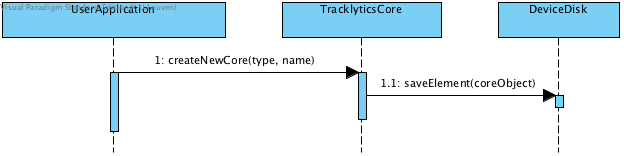
\includegraphics[scale=0.4]{Afbeeldingen/Architectuur/FlowDiagram1}
  \caption{Flow diagram 1.}
  \label{fig:flow1}
\end{figure}
\begin{figure}[!h]
  \centering
  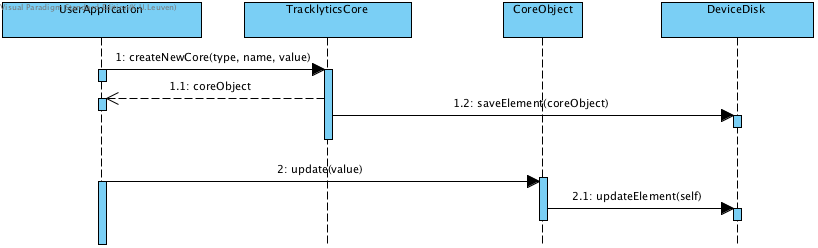
\includegraphics[scale=0.4]{Afbeeldingen/Architectuur/FlowDiagram2}
  \caption{Flow diagram 2.}
  \label{fig:flow2}
\end{figure}

Het monitoren van de gegevens van de applicatie kan opgesplitst worden in twee verschillende flows. \\

De eerste flow \ref{fig:flow1} toont de meest simpele flow. De developer geeft aan dat een bepaalde waarde gecollecteerd moet worden. De TracklyticsCore slaat deze informatie op op de schijf van het toestel van de gebruiker, zodat deze later verwerkt kan worden. De verwerking van de data wordt uitgelegd in de volgende sectie \ref{sec:VerzendenEnOpslaanVanGegevens}. Deze situatie is geldig in de gevallen dat de developer data voor een histogram of een gauge wil collecteren. De uitleg over deze componenten staat in het volgende hoofdstuk \ref{sec:Klassediagram}.\\

De tweede flow \ref{fig:flow2} toont een uitgebreidere flow van de vorige flow. Er wordt weer een bepaalde waarde gecollecteerd en deze wordt opgeslagen op de harde schijf van het toestel. Bij deze flow wordt een Core Object terug gegeven waar verdere acties mee mogelijk zijn. Deze acties worden gebundeld in de \texttt{update} call. Deze flow is geldig als de developer data voor een Counter, een Timer of een Meter wil collecteren. De uitleg over deze componenten en de acties die op deze componenten mogelijk zijn staan in het volgende hoofdstuk \ref{sec:Klassediagram} \\


\subsection{Verzenden en opslaan van de gegevens} \label{sec:VerzendenEnOpslaanVanGegevens}
In het volgende diagram \ref{fig:flow3} wordt getoond hoe het verzenden van de gegevens van het toestel naar de server in zijn werk gaat en hoe de gegevens worden opgeslagen in de database. \\
\begin{figure}[!h]
  \centering
  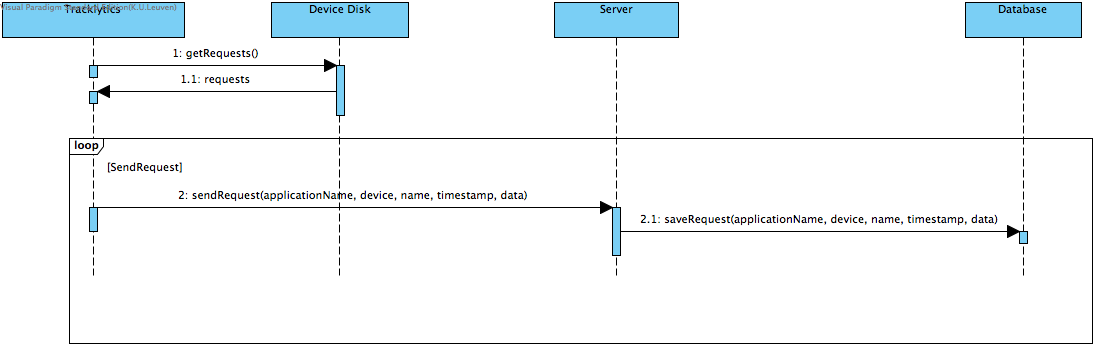
\includegraphics[scale=0.4]{Afbeeldingen/Architectuur/FlowDiagram3}
  \caption{Flow diagram 3.}
  \label{fig:flow3}
\end{figure}


De Tracklytics library haalt eerst alle meetgegevens van de harde schijf van het mobiele toestel. De Tracklytics library synchroniseert hierna alle meetgegevens naar de Tracklytics backend. De server waar de request terecht komt verwerkt deze gegevens en slaat deze op in de database. Nadat de server antwoord heeft gegeven aan de Tracklytics library dat de request succesvol behandelt is, verwijdert de library dit meetgegeven van de harde schijf. Indien de server antwoordt dat de operatie mislukt is, dan mag dit meetgegeven niet verwijdert worden zoals eerder besproken.







%%% Local Variables: 
%%% mode: latex
%%% TeX-master: "masterproef"
%%% End: 
